\chapter{Interaktionsdesign}
\section{Analyse}
In diesem Abschnitt soll analysiert werden, wie die möglichen Interaktionen gestaltet sind. Werden die Designprinzipien Normans (Kap. \ref{sec:interactionDesign}) nicht hinreichend erfüllt, lässt dies auf ein zu behebendes Problem der User-Experience schließen.
Da es sich bei \textit{FalkoFX} um eine bestehende Anwendung in der Entwicklungsphase handelt, ist bereits ein implizites Interaktionskonzept gegeben.\par
Die Anwendung besteht im Wesentlichen aus drei Bereichen. Der erste Bereich ist die \textbf{Navigation}, die sich am oberen Rand des Fensters befindet. Hier werden zusätzlich zu den Navigationselementen Hilfetexte eingeblendet. Das zweite Areal, genannt \textbf{Sidebar}, ist an der rechten Seite der Applikation untergebracht und stellt weitergehende Informationen und Interaktionsmöglichkeiten für den aktuell angezeigten Bildschirm zur Verfügung. Der letzte und größte Bereich ist der \textbf{Content}-Bereich. Er nimmt den übrig gebliebenen Platz ein. Hier werden die Hauptinformationen und Bedienelemente dargestellt.\par
\begin{figure}[H]
 \centering
 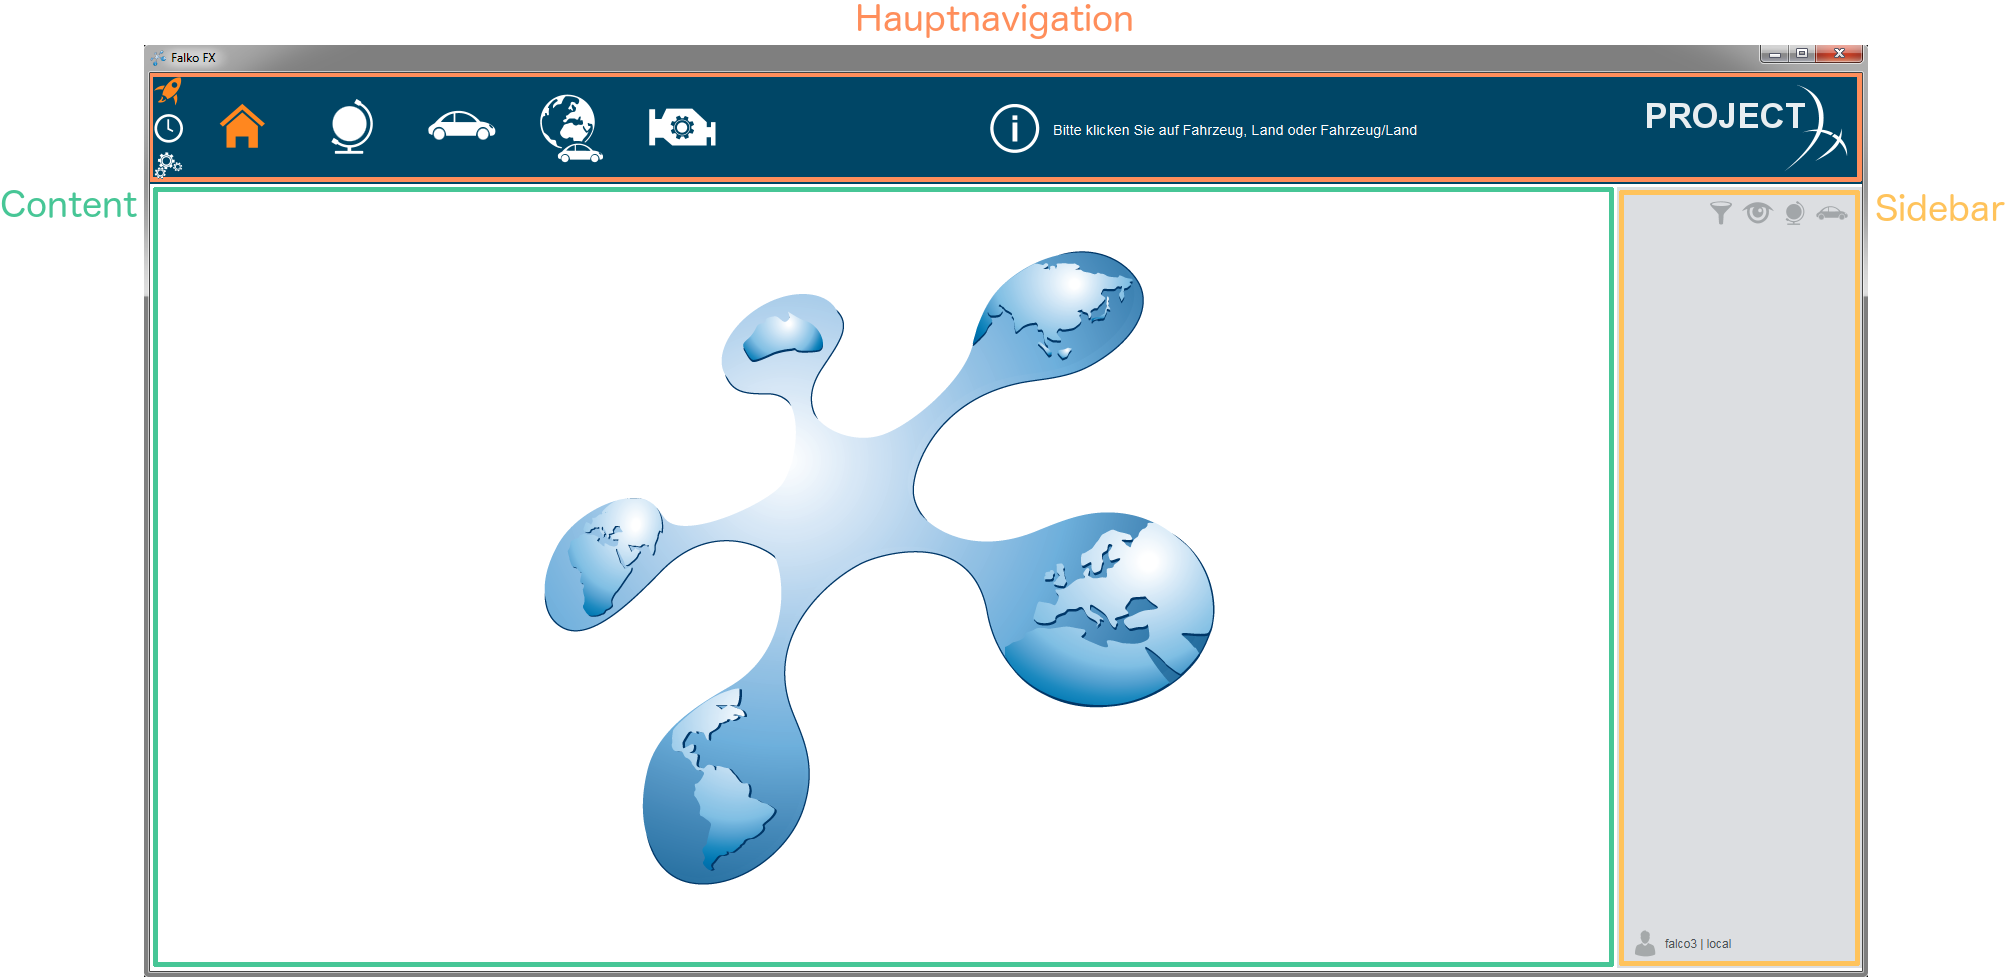
\includegraphics[width=0.8\textwidth]{grafiken/areas.png}
 \caption{Bereiche in FalkoFX}
 \label{fig:areas}
\end{figure}
Das Konzept der gemeinsamen Region wird hier durch die verschiedenen Hintergrundfarben realisiert und unterstreicht die unterschiedlichen Funktionalitäten.\par
\heading{Navigation}
Im Navigationsbereich findet sich im initialen Zustand die Hauptnavigation wieder. Durch die Bedienelemente an der linken Seite der Leiste kann zwischen folgenden Funktionen gewechselt werden:
\begin{enumerate}
	\item Hauptnavigation: Wechsel zwischen Standard-Anwendungsfällen und der verschiedenen Ansichten
	\item Versionsvergleich: Navigation für Anwendungsfälle mit Versionsvergleich
	\item Einstellungen: Menü zum Ändern anwendungsspezifischer Einstellungen
\end{enumerate}
\begin{figure}[H]
 \centering
 
\includegraphics[width=0.05\textwidth]{grafiken/ribbon.png}
 \caption{Umschalten der Navigation}
 \label{fig:ribbon}
\end{figure}
Durch die vertikale Orientierung, der geringeren Größe und der Nähe zueinander heben sich die Elemente zum Umschalten der Navigation deutlich von den andren Schaltflächen ab. Wird eines der Elemente angewählt, wird eine Aktion ausgeführt und die Kindelemente, falls vorhanden, werden mittels Animation sichtbar. Die nachfolgenden Elemente der höher liegenden Ebenen werden \enquote{zur Seite geschoben}.\par
\begin{figure}[H]
 \centering
 
\includegraphics[width=0.85\textwidth]{grafiken/navi.png}
 \caption{Navigationshierarchie}
 \label{fig:navi}
\end{figure}
Die Elemente einer einzigen Navigationsebene benötigen keine weitere Trennung. Durch den Freiraum zwischen diesen ist eine hinreichende Trennung erwirkt. Zwischen den verschiedenen Ebenen wird zusätzlich zu einer Farbabstufung eine weiße Trennlinie eingeblendet, die auf der linken Seite einen angedeuteten Pfeil enthält , der die Navigationshierarchie verdeutlicht. Dazu trägt ebenfalls die bereits erwähnte Animation bei.\par
Das Piktogramm des selektierten Navigationselementes wird orange eingefärbt, um die Orientierung zu gewährleisten. Kann der Nutzer eine bestimmte Interaktion nicht ausführen, erscheint das Icon grau.\par
Durch das Anklicken eines Icons wird der neue Bildschirm angezeigt. Dies geht oft mit dem Laden von Daten einher. Sollten Daten aus der Datenbank geladen werden müssen, wird währenddessen eine Ladeanimation angezeigt. Andernfalls wird der Bildschirm in weniger als 500 Millisekunden angezeigt, wodurch kein weiteres Feedback von Nöten ist. Im Gegenteil: Eine kurz aufblitzende Ladeanimation würde den Anwender eher irritieren als unterstützen.\par
Den Einstieg in jeden Anwendungsfall bietet der Filter. Der Filter besteht in der simpelsten Variante aus folgenden Komponenten:
\begin{itemize}
	\item \textbf{Radial-Menü:} Ein rundes Menü, in dem die zu filternden Attribute ausgewählt werden können
	\item \textbf{Multi-Level-Liste:} Eine mehrstufige Liste mit Suchfunktion, aus der Werte zu den Attributen angewählt werden können
	\item \textbf{Filterselektion:} Eine Liste, welche die aktuell ausgewählten Werte gruppiert darstellt und das Abwählen dieser Werte erlaubt
\end{itemize}
\begin{figure}[H]
 \centering
 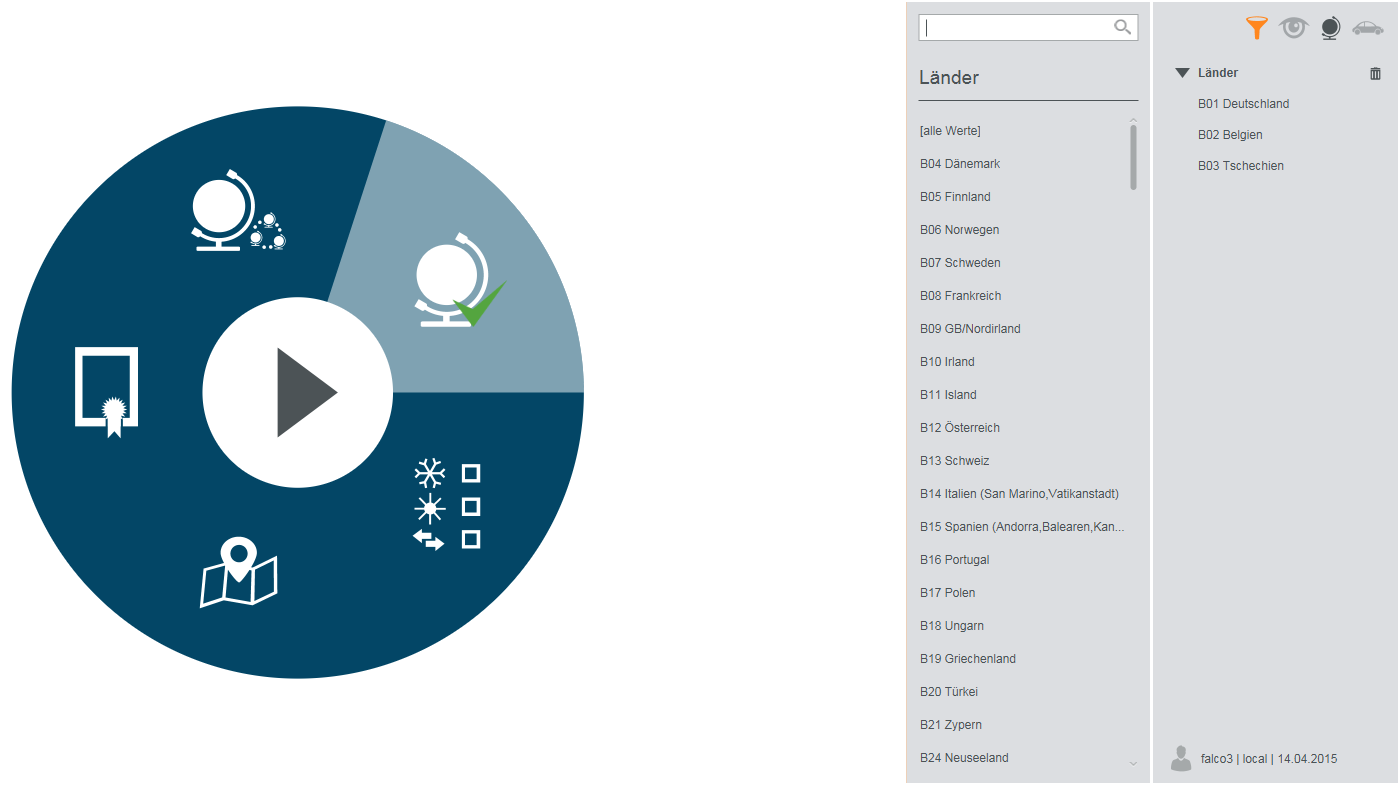
\includegraphics[width=0.6\textwidth]{grafiken/filter_short.png}
 \caption{Beispiel Filter}
 \label{fig:filter}
\end{figure}
Im Radial-Menü sind die Elemente kreisförmig um einen \textit{Play}-Button angeordnet, der standardmäßig deaktiviert ist. Erst, wenn die Ergebnismenge, die durch die gefilterten Attributwerte erzeugt wird, valide ist, wird der Button und das dazugehörige Navigationselement in der Navigationsleiste aktiviert. Die aktuelle Selektion in dem Menü wird durch einen helleren Kreisausschnitt über dem entsprechenden Element markiert. So wird dieser Bereich deutlich hervorgehoben.\par
Die Multi-Level-Liste enthält Werte, die als Filterkriterium ausgewählt werden können. Einige dieser Werte gruppieren weitere Werte und können nicht übernommen werden. Stattdessen öffnet sich beim Auswählen dieser Elemente eine untergeordnete Ebene der Multi-Level-Liste. Diese Werte sind mit einem Pfeil markiert, der in die gleiche Richtung zeigt, in die auch die nachfolgende Animation verläuft.\par
\begin{itemize}
	\item \textbf{Radial-Menü:} Ein rundes Menü, in dem die zu filternden Attribute ausgewählt werden können
	\item \textbf{Multi-Level-Liste:} Eine mehrstufige Liste mit Suchfunktion, aus der Werte zu den Attributen angewählt werden können
	\item \textbf{Filterselektion:} Eine Liste, welche die aktuell ausgewählten Werte gruppiert darstellt und das Abwählen dieser Werte erlaubt
\end{itemize}
\begin{figure}[H]
 \centering
 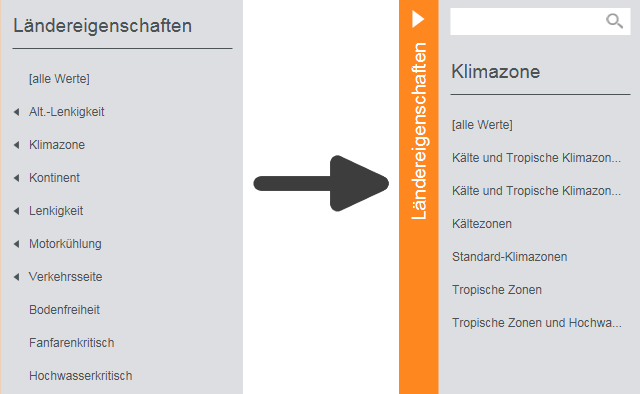
\includegraphics[width=0.4\textwidth]{grafiken/mll_combined.png}
 \caption{Multi-Level-Liste}
 \label{fig:mll}
\end{figure}
Nach dem Filtern der Daten lassen sich die Ergebnisansichten öffnen. Eine mögliche Präsentation ist die Tabellenansicht. Es handelt sich hierbei um eine komplexe Tabelle, die sämtliche Informationen darstellt. Die Spalten entsprechen den Attributen, zu denen erlaubte Werte im Filter ausgewählt wurden. Zusätzlich sind diese Attribute gruppiert. Die Trennung der Gruppen erfolgt durch deutlich sichtbare Linien, die vertikal zwischen den Spalten der einzelnen Gruppen verlaufen. Die einzelnen Gruppen lassen sich über Bedienelemente in der Sidebar aus- und einblenden, sowie per Drag\& Drop-Geste in der Reihenfolge vertauschen. Der um 45$^{\circ}$ geneigte Spaltenkopf sorgt für eine kompaktere Darstellung, da die minimale Spaltenbreite so nicht mehr durch den Titel der Spalte bestimmt wird. Besonders hilfreich ist diese Präsentation der Spaltenköpfe bei Werten, die nur sehr kurze Bezeichner annehmen. Der Beginn der gedrehten Beschriftungen ist dabei auf einer gedachten horizontalen Linie angeordnet. Auch in diesem Fall lässt sich das Gesetz der Kontinuität anwenden, wodurch die Überschriften als eine zusammengehörige Einheit wahrgenommen werden.\par
\begin{figure}[H]
 \centering
 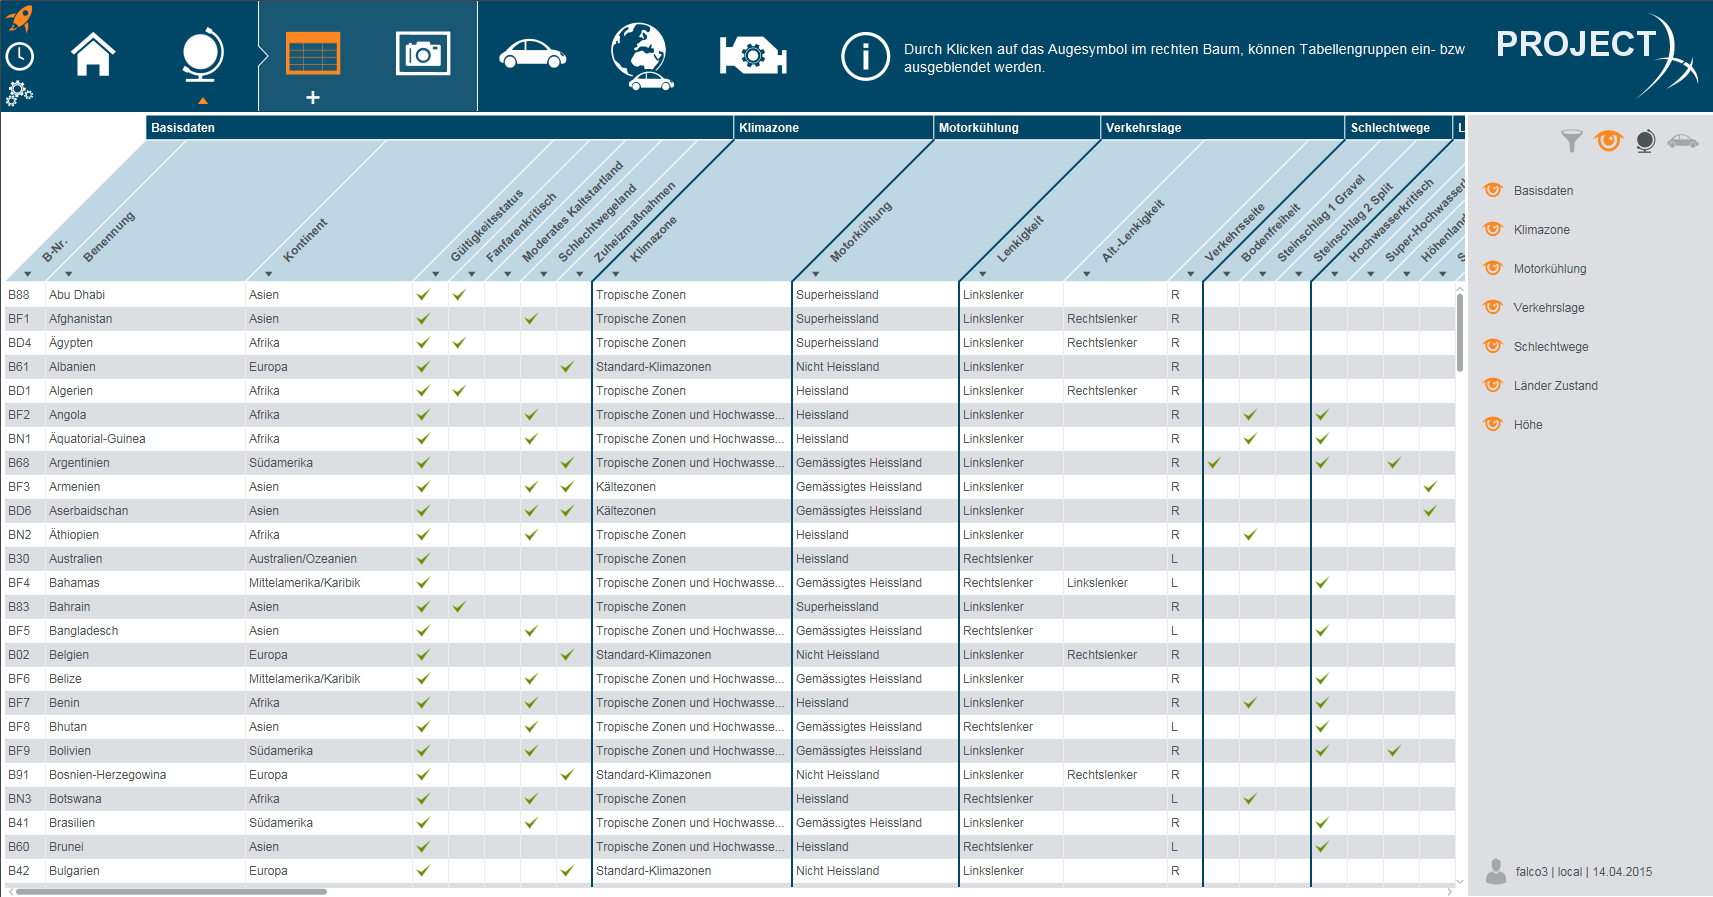
\includegraphics[width=0.6\textwidth]{grafiken/full_result_table.png}
 \caption{Ergebnistabelle}
 \label{fig:resultTable}
\end{figure}
Über die Pfeile im Spaltenkopf lässt sich ein \textit{Overlay} einblenden, in dem die präsentierten Daten auf einfache Weise zusätzlich eingeschränkt werden können, falls mit den aktuellen Einstellungen mehr Datensätze als gewünscht angezeigt werden. Zwar könnten die Pfeile als Elemente zur Umsortierung missverstanden werden, allerdings ist dies kein kritisches Problem, da sich das Overlay nach kurzer Zeit (oder nach dem Verlassen des Bereiches mit dem Mauscursor) schließt und andere Schaltflächen während der Anzeige nicht blockiert werden.\par
\begin{figure}[H]
 \centering
 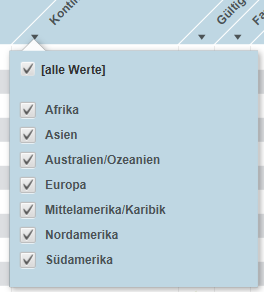
\includegraphics[width=0.3\textwidth]{grafiken/overlay.png}
 \caption{Schnellfilter-Overlay}
 \label{fig:autofilter}
\end{figure}
Im Navigationsbereich ist unter der Schaltfläche der Ergebnispräsentation ein zusätzliches Icon (\ding{58}) aufgetaucht. Bei Klick auf den Bereich des zusätzlichen Icons öffnet sich, mit einer \enquote{Aufklapp-} Animation ein untergeordnetes Menü, das erweiterte Optionen für die derzeit aktive Ansicht bereitstellt. Darunter fallen die Export-Möglichkeiten in PDF und Excel. Die Animation verdeutlicht die Zugehörigkeit zu dem Menüpunkt des aktuell ausgewählten Elements. Als ein mögliches Problem könnte sich das Auftauchen des Icons erweisen. Da der Menüpunkt schon vorher sichtbar war, wird die Änderung ggf. nicht wahrgenommen und ignoriert. Es wird also das Prinzip der Sichtbarkeit nicht vollständig erfüllt.\par
Eine weitere mögliche Ergebnispräsentation ist die Galerie. Hier werden im oberen Bereich Vorschaubilder für Daten angezeigt und darunter eine Detailansicht zum aktuell ausgewählten Element. Mit der Hilfe von $\blacktriangleright$ - und $\blacktriangleleft$ - Schaltflächen lassen sich die Objekte animiert durchschalten. Die aktuelle Selektion wird dadurch verdeutlicht, dass sich dass entsprechende Element stets mittig über der Detailansicht befindet. Zusätzlich wird ein Bezeichner in orangener Schrift darüber angezeigt und das Element wird durch Vergrößerung hervorgehoben. Alle anderen Elemente rücken durch eine geringe Opazität (\enquote{Deckkraft}) in den Hintergrund. Das Gesetz der Prägnanz wird hier durch mehrere ausschlaggebende Faktoren erfüllt und zeigt dem Anwender unmissverständlich die aktuelle Selektion an. \par
\begin{figure}[H]
 \centering
 \setlength{\fboxsep}{0pt}
 \setlength{\fboxrule}{0.5pt}
 \fbox{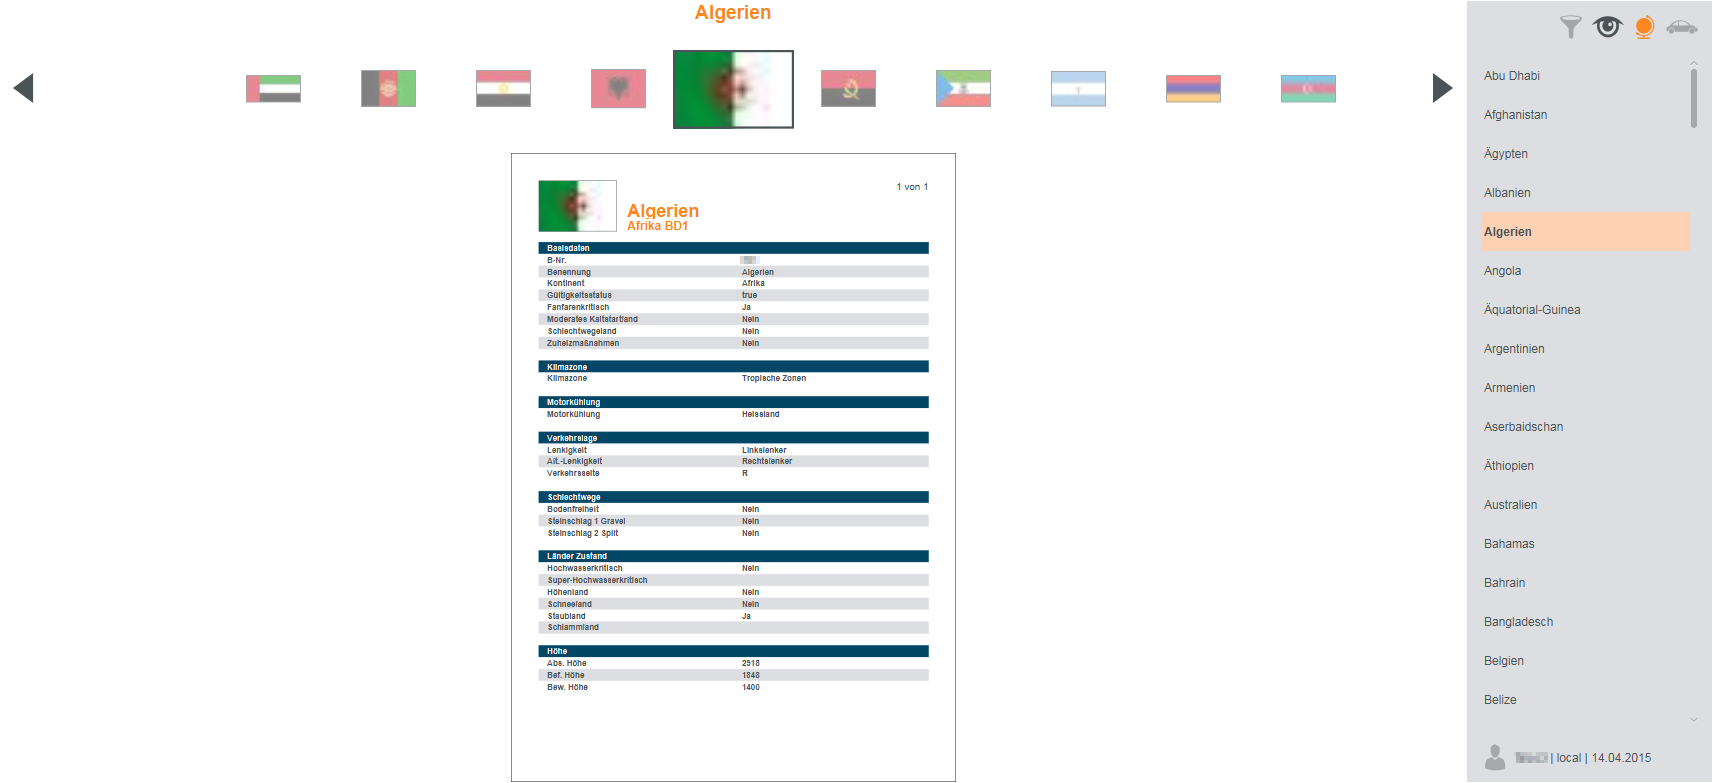
\includegraphics[width=0.6\textwidth]{grafiken/gallery.png}}
 \caption{Galerie}
 \label{fig:gallery}
\end{figure}
Für diese Ansicht ist in der Sidebar standardmäßig die \textit{Ergebnisvorschau} eingeblendet. Diese Ansicht bietet einen Überblick über alle Datensätze, die den Filterkriterien entsprechen. Die Selektion in dieser Liste ist mit der Selektion der Galerie-Komponente gekoppelt und wird so synchron gehalten. Auch die \textit{Ansichtskonfiguration}, die bereits aus der Tabellenansicht bekannt ist, kann hier angewählt und verändert werden. Daraufhin ändern sich die in der Detailansicht der Galerie dargestellten Attributgruppen.\par
Ein Klick auf die Detailansicht öffnet eine vergrößerte Darstellung, den sogenannten \textit{Lesemodus}. Er bietet die Möglichkeit, die zuvor dargestellten Informationen durch die größere Darstellung besser lesen zu können. Die vorherigen und Nachfolgenden Datensätze werden durch perspektivisch verschobene Seiten links und rechts der aktuell selektierten Seite eingeblendet. Durch Anklicken lassen sich diese, ebenfalls animiert, in den Vordergrund holen, während die aktive Seite \enquote{wegblättert}. Im Hintergrund verändert sich das selektierte Element in der Galerie. Durch das Anklicken des Tür-Icons in der unteren rechten Ecke lässt sich der Lesemodus wieder schließen.\par
\begin{figure}[H]
 \centering
 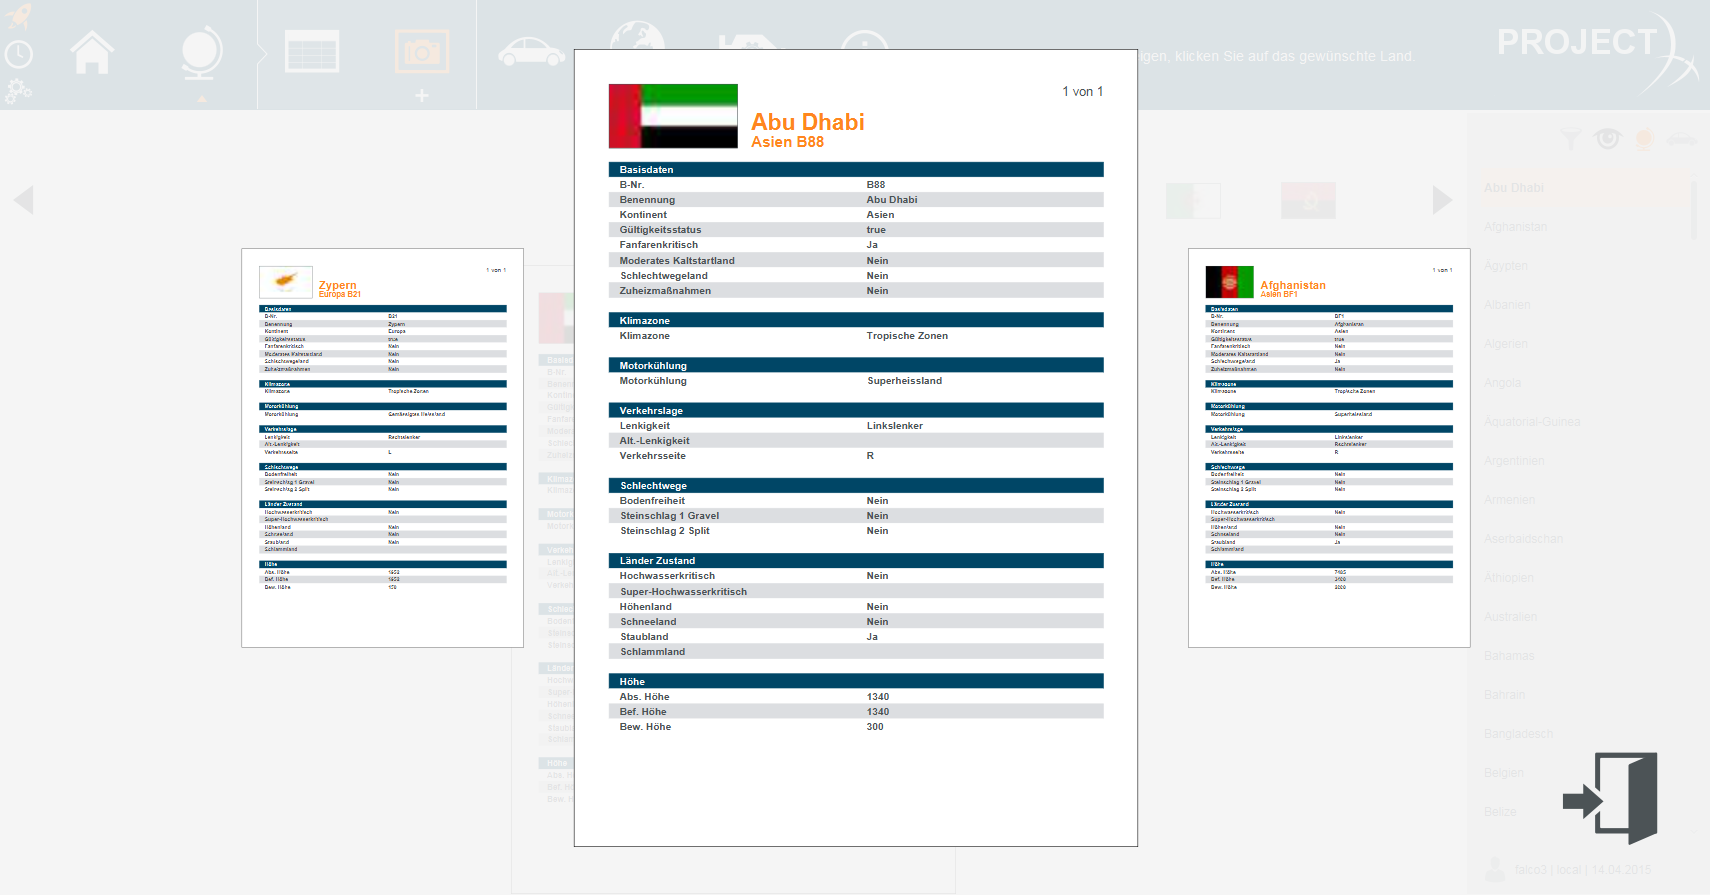
\includegraphics[width=0.6\textwidth]{grafiken/readmode.png}
 \caption{Lesemodus}
 \label{fig:readmode}
\end{figure}
\subsection{Tastaturbedienbarkeit}
\subsection{Übertragung von Touchgesten auf Maussteuerung}
Mit Blick auf den immer stärker werdenden Trend, auch Geschäftsanwendungen auf mobile Geräte zu portieren, soll an dieser Stelle geprüft werden, inwiefern die Touchgesten (vgl. \ref{fig:touchGestures}) auf das Bedienkonzept am Desktop-PC übertragbar sind. Dies soll zum einen zu einer intuitiveren Bedienung mit der Maus beitragen und zum anderen für die Benutzung der Software auf sogenannten Convertibles vorsorgen.\par%Erklärung Convertibles
Der Mauszeiger wird zu diesem Zweck als \enquote{Ersatz} für den Finger auf einem Touch-Display verwendet. Da es nur einen Mauszeiger und eine Maus gibt, ist es technisch gesehen nur möglich, Gesten durchzuführen, die genau einen Finger benötigen. Dies sind \textit{Tap}, \textit{Double Tap}, \textit{Drag}, \textit{Flick} und \textit{Press}. Die \textit{Tap} und \textit{Double Tap}-Gesten entsprechen sowohl von der Durchführung, als auch von der Semantik in der Regel dem einfachen Mausklick bzw. dem Doppelklick. Die \textit{Drag}-Geste ist der Drag\& Drop Aktion der Maus sehr ähnlich. An vielen Stellen jedoch, an denen bei mobilen Anwendungen \textit{Drag}-Gesten verwendet werden würden, wird die Benutzung eines UI-Elements auf dem Desktop-PC mit anderen Mitteln gelöst. Für den \textit{Flick}, auch \textit{Swipe} genannt, existiert kein Pendant im Pensum der normalen Maus- und Tastatur- Interaktion. Dennoch ist es denkbar, eine solche Geste mit einer schnell ausgeführten Drag\& Drop-Aktion zu ermöglichen. Auch der \textit{Press} könnte mit den gegebenen Eingabemitteln umgesetzt werden. Eine solche Aktion ist jedoch in den meisten Fällen nur bedingt intuitiv verwendbar, da keine ähnlichen, dem Nutzer vertrauten, Aktionen für die Maussteuerung existieren. Als Ersatz kann der Rechtsklick bei der Desktop-Verwendung genutzt werden.\par

\section{Design}
\subsection{•}
\section{Implementierung} \label{sec:interactionImplementation}
